\documentclass[dvipdfmx]{jsarticle}
\setcounter{section}{1}
\setcounter{subsection}{1}
\usepackage{xr}
\externaldocument{3.1.1}
\usepackage{amsmath,amsfonts,amssymb,array,comment,mathtools,url,docmute}
\usepackage{longtable,booktabs,dcolumn,tabularx,mathtools,multirow,colortbl,xcolor}
\usepackage[dvipdfmx]{graphics}
\usepackage{bmpsize}
\usepackage{amsthm}
\usepackage{enumitem}
\setlistdepth{20}
\renewlist{itemize}{itemize}{20}
\setlist[itemize]{label=•}
\renewlist{enumerate}{enumerate}{20}
\setlist[enumerate]{label=\arabic*.}
\setcounter{MaxMatrixCols}{20}
\setcounter{tocdepth}{3}
\newcommand{\rotin}{\text{\rotatebox[origin=c]{90}{$\in $}}}
\renewcommand{\thesection}{第\arabic{section}部}
\renewcommand{\thesubsection}{\arabic{section}.\arabic{subsection}}
\renewcommand{\thesubsubsection}{\arabic{section}.\arabic{subsection}.\arabic{subsubsection}}
\everymath{\displaystyle}
\allowdisplaybreaks[4]
\usepackage{vtable}
\theoremstyle{definition}
\newtheorem{thm}{定理}[subsection]
\newtheorem*{thm*}{定理}
\newtheorem{dfn}{定義}[subsection]
\newtheorem*{dfn*}{定義}
\newtheorem{axs}[dfn]{公理}
\newtheorem*{axs*}{公理}
\renewcommand{\headfont}{\bfseries}
\makeatletter
  \renewcommand{\section}{%
    \@startsection{section}{1}{\z@}%
    {\Cvs}{\Cvs}%
    {\normalfont\huge\headfont\raggedright}}
\makeatother
\makeatletter
  \renewcommand{\subsection}{%
    \@startsection{subsection}{2}{\z@}%
    {0.5\Cvs}{0.5\Cvs}%
    {\normalfont\LARGE\headfont\raggedright}}
\makeatother
\makeatletter
  \renewcommand{\subsubsection}{%
    \@startsection{subsubsection}{3}{\z@}%
    {0.4\Cvs}{0.4\Cvs}%
    {\normalfont\Large\headfont\raggedright}}
\makeatother
\makeatletter
\renewenvironment{proof}[1][\proofname]{\par
  \pushQED{\qed}%
  \normalfont \topsep6\p@\@plus6\p@\relax
  \trivlist
  \item\relax
  {
  #1\@addpunct{.}}\hspace\labelsep\ignorespaces
}{%
  \popQED\endtrivlist\@endpefalse
}
\makeatother
\renewcommand{\proofname}{\textbf{証明}}
\usepackage{tikz,graphics}
\usepackage[dvipdfmx]{hyperref}
\usepackage{pxjahyper}
\hypersetup{
 setpagesize=false,
 bookmarks=true,
 bookmarksdepth=tocdepth,
 bookmarksnumbered=true,
 colorlinks=false,
 pdftitle={},
 pdfsubject={},
 pdfauthor={},
 pdfkeywords={}}
\begin{document}
%\hypertarget{ux7fa4ux6e96ux540cux578bux5199ux50cf}{%
\subsection{群準同型写像}%\label{ux7fa4ux6e96ux540cux578bux5199ux50cf}}
%\hypertarget{ux7fa4ux6e96ux540cux578bux5199ux50cf-1}{%
\subsubsection{群準同型写像}%\label{ux7fa4ux6e96ux540cux578bux5199ux50cf-1}}
\begin{dfn}
2つの群々$\left( G,*_{G} \right)$、$\left( H,*_{H} \right)$について、写像$f:G \rightarrow H$が、$\forall a,b \in G$に対し、次式を満たすとき、この写像$f$をその群$\left( G,*_{G} \right)$からその群$\left( H,*_{H} \right)$への群準同型写像という。
\begin{align*}
f:G \rightarrow H;f\left( a*_{G}b \right) \mapsto f(a)*_{H}f(b)
\end{align*}
\end{dfn}
\begin{thm}\label{3.1.2.1}
2つの群々$\left( G,*_{G} \right)$、$\left( H,*_{H} \right)$の間の群準同型写像$f:G \rightarrow H$について、次のことが成り立つ。
\begin{itemize}
\item
  $f\left( 1_{\left( G,*_{G} \right)} \right) = 1_{\left( H,*_{H} \right)}$が成り立つ。
\item
  $\forall a \in G$に対し、$f\left( a^{- 1} \right) = {f(a)}^{- 1}$が成り立つ。
\end{itemize}
\end{thm}
\begin{proof}
2つの群々$\left( G,*_{G} \right)$、$\left( H,*_{H} \right)$の間の群準同型写像$f:G \rightarrow H$について、次のようになる。
\begin{align*}
f\left( 1_{\left( G,*_{G} \right)} \right) &= f\left( 1_{\left( G,*_{G} \right)} \right)*_{H}1_{\left( H,*_{H} \right)}\\
&= f\left( 1_{\left( G,*_{G} \right)} \right)*_{H}f\left( 1_{\left( G,*_{G} \right)} \right)*_{H}f\left( 1_{\left( G,*_{G} \right)} \right)^{- 1}\\
&= f\left( 1_{\left( G,*_{G} \right)}*_{G}1_{\left( G,*_{G} \right)} \right)*_{H}f\left( 1_{\left( G,*_{G} \right)} \right)^{- 1}\\
&= f\left( 1_{\left( G,*_{G} \right)} \right)*_{H}f\left( 1_{\left( G,*_{G} \right)} \right)^{- 1}\\
&= 1_{\left( H,*_{H} \right)}
\end{align*}\par
また、$\forall a \in G$に対し、次のようになる。
\begin{align*}
f\left( a^{- 1} \right) &= f\left( a^{- 1} \right)*_{H}1_{\left( H,*_{H} \right)}\\
&= f\left( a^{- 1} \right)*_{H}f(a)*_{H}{f(a)}^{- 1}\\
&= f\left( a^{- 1}*_{G}a \right)*_{H}{f(a)}^{- 1}\\
&= f\left( 1_{\left( G,*_{G} \right)} \right)*_{H}{f(a)}^{- 1}\\
&= 1_{\left( H,*_{H} \right)}*_{H}{f(a)}^{- 1}\\
&= {f(a)}^{- 1}
\end{align*}
\end{proof}
\begin{thm}\label{3.1.2.2}
3つの群々$\left( G,*_{G} \right)$、$\left( H,*_{H} \right)$、$\left( I,*_{I} \right)$の間の2つの群準同型写像たち$f:G \rightarrow H$、$g:H \rightarrow I$の合成写像$g \circ f$も群準同型写像である。
\end{thm}
\begin{proof}
3つの群々$\left( G,*_{G} \right)$、$\left( H,*_{H} \right)$、$\left( I,*_{I} \right)$の間の2つの群準同型写像たち$f:G \rightarrow H$、$g:H \rightarrow I$が与えられたとき、$\forall a,b \in G$に対し、次のようになる。
\begin{align*}
g \circ f\left( a*_{G}b \right) &= g\left( f\left( a*_{G}b \right) \right)\\
&= g\left( f(a)*_{H}f(b) \right)\\
&= g\left( f(a) \right)*_{I}g\left( f(b) \right)\\
&= g \circ f(a)*_{I}g \circ f(b)
\end{align*}
\end{proof}
%\hypertarget{ux7fa4ux540cux578bux5199ux50cf}{%
\subsubsection{群同型写像}%\label{ux7fa4ux540cux578bux5199ux50cf}}
\begin{dfn}
群準同型写像のうち、全射であるもの、単射であるもの、全単射であるものをそれぞれ全射群準同型写像、単射群準同型写像、群同型写像という。
\end{dfn}
\begin{thm}\label{3.1.2.3}
2つの群々$\left( G,*_{G} \right)$、$\left( H,*_{H} \right)$の間の群同型写像$f:G\overset{\sim}{\rightarrow}H$の逆写像$f^{- 1}$も群同型写像である。
\end{thm}
\begin{proof}
2つの群々$\left( G,*_{G} \right)$、$\left( H,*_{H} \right)$の間の群同型写像$f:G\overset{\sim}{\rightarrow}H$の逆対応$f^{- 1}$は写像でその逆写像$f^{- 1}$も全単射$f^{- 1}:H\overset{\sim}{\rightarrow}G$であり、$\forall a,b \in H$に対し、次のようになる。
\begin{align*}
f^{- 1}\left( a*_{H}b \right) &= f^{- 1}\left( f \circ f^{- 1}(a)*_{H}f \circ f^{- 1}(b) \right)\\
&= f^{- 1}\left( f\left( f^{- 1}(a) \right)*_{H}f\left( f^{- 1}(b) \right) \right)\\
&= f^{- 1}\left( f\left( f^{- 1}(a)*_{G}f^{- 1}(b) \right) \right)\\
&= f^{- 1} \circ f\left( f^{- 1}(a)*_{G}f^{- 1}(b) \right)\\
&= f^{- 1}(a)*_{G}f^{- 1}(b)
\end{align*}
\end{proof}
\begin{dfn}
2つの群々$\left( G,*_{G} \right)$、$\left( H,*_{H} \right)$は、その集合$G$からその集合$H$への群同型写像$f:G\overset{\sim}{\rightarrow}H$が存在するとき、群同型であるといい$\left( G,*_{G} \right) \cong \left( H,*_{H} \right)$と書く。
\end{dfn}
\begin{thm}\label{3.1.2.4}
次のことが成り立つ、即ち、その関係$\cong$は同値関係である。
\begin{itemize}
\item
  $\left( G,*_{G} \right) \cong \left( G,*_{G} \right)$が成り立つ。
\item
  $\left( G,*_{G} \right) \cong \left( H,*_{H} \right)$が成り立つなら、$\left( H,*_{H} \right) \cong \left( G,*_{G} \right)$も成り立つ。
\item
  $\left( G,*_{G} \right) \cong \left( H,*_{H} \right)$かつ$\left( H,*_{H} \right) \cong \left( I,*_{I} \right)$が成り立つなら、$\left( G,*_{G} \right) \cong \left( I,*_{I} \right)$も成り立つ。
\end{itemize}
\end{thm}\par
これにより、群同型な2つの群々$\left( G,*_{G} \right)$、$\left( H,*_{H} \right)$を考えるとき、その集合$G$からその集合$H$への群同型写像$f:G\overset{\sim}{\rightarrow}H$を用いれば、その集合$G$がその集合$H$に、その集合$G$の任意の元$a$がその集合$H$のある元$f(a)$に、その算法$*_{G}$からその算法$*_{H}$に名前の付け替えただけで、群としての構造が保たれることができる。
\begin{proof}
群同型な3つの群々$\left( G,*_{G} \right)$、$\left( H,*_{H} \right)$、$\left( I,*_{I} \right)$が与えられたとする。\par
その集合$G$の恒等写像$I_{G}$を考えると、次のようになり、
\begin{align*}
I_{G}\left( a*_{G}b \right) = a*_{G}b = I_{G}(a)*_{G}I_{G}(b)
\end{align*}
恒等写像の逆写像はもとのその恒等写像自身であるので、この写像$I_{G}$は群同型写像である。よって、$\left( G,*_{G} \right) \cong \left( G,*_{G} \right)$が成り立つ。\par
$\left( G,*_{G} \right) \cong \left( H,*_{H} \right)$が成り立つなら、その群$\left( G,*_{G} \right)$からその群$\left( H,*_{H} \right)$への群同型写像$f$が存在し、群同型写像の逆対応は群同型写像であったので、その集合$H$からその集合$G$への群同型写像が存在し$\left( H,*_{H} \right) \cong \left( G,*_{G} \right)$が成り立つ。\par
$\left( G,*_{G} \right) \cong \left( H,*_{H} \right)$かつ$\left( H,*_{H} \right) \cong \left( I,*_{I} \right)$が成り立つなら、その群$\left( G,*_{G} \right)$からその群$\left( H,*_{H} \right)$への群同型写像$f$が存在するかつ、その群$\left( H,*_{H} \right)$からその群$\left( I,*_{I} \right)$への群同型写像$g$が存在し、定理\ref{3.1.2.2}よりその写像$g \circ f$も群準同型写像であり、定理\ref{3.1.2.3}よりこれらの逆写像たち$f^{- 1}$、$g^{- 1}$も群同型写像たちであり、さらに、その合成写像$f^{- 1} \circ g^{- 1}$も群準同型写像である。ここで、次のようになるので、
\begin{align*}
(g \circ f) \circ \left( f^{- 1} \circ g^{- 1} \right) &= g \circ \left( f \circ f^{- 1} \right) \circ g^{- 1}\\
&= g \circ I_{H} \circ g^{- 1}\\
&= g \circ g^{- 1} = I_{I}\\
\left( f^{- 1} \circ g^{- 1} \right) \circ (g \circ f) &= f^{- 1} \circ \left( g^{- 1} \circ g \right) \circ f\\
&= f^{- 1} \circ I_{H} \circ f\\
&= f^{- 1} \circ f = I_{G}
\end{align*}
その写像$f^{- 1} \circ g^{- 1}$はその写像$g \circ f$の逆写像でありその写像$g \circ f$は群同型写像となる。よって、$\left( G,*_{G} \right) \cong \left( I,*_{I} \right)$が成り立つ。
\end{proof}
\begin{thm}\label{3.1.2.5}
2つの群々$\left( G,*_{G} \right)$、$\left( H,*_{H} \right)$の間の群準同型写像$f:G \rightarrow H$の値域$V(f)$を用いた群$\left( V(f),*_{H} \right)$はその群$\left( H,*_{H} \right)$の部分群である。
\end{thm}
\begin{proof}
2つの群々$\left( G,*_{G} \right)$、$\left( H,*_{H} \right)$の間の群準同型写像$f:G \rightarrow H$について、$f\left( 1_{\left( G,*_{G} \right)} \right) = 1_{\left( H,*_{H} \right)}$が成り立つのであったので、$1_{\left( H,*_{H} \right)} \in V(f)$が成り立つ。\par
また、$\forall f(a),f(b) \in V(f)$に対し、$a,b \in G$なる元々$a$、$b$が存在し、$f\left( a*_{G}b \right) = f(a)*_{H}f(b) \in H$が成り立つかつ、$\forall f(a) \in V(f)$に対し、$a \in G$なる元$a$、さらに、これの逆元$a^{- 1}$がその集合$G$に存在し、定理\ref{3.1.2.1}より$f\left( a^{- 1} \right) = {f(a)}^{- 1}$が成り立つのであったので、${f(a)}^{- 1} = f\left( a^{- 1} \right) \in V(f)$が成り立つ。\par
以上より、定理\ref{3.1.1.6}よりその群$\left( H,*_{H} \right)$をなすその集合$H$のその部分集合$V(f)$がその算法$*_{H}$に関して部分群$\left( V(f),*_{H} \right)$をなす。
\end{proof}
\begin{dfn}
2つの群々$\left( G,*_{G} \right)$、$\left( H,*_{H} \right)$について、ある単射群準同型写像$f:G \rightarrowtail H$が与えられたとき、その写像$f$の終集合を$V(f)$とおいた写像$f':G \rightarrowtail V(f)$は明らかに全射であるので、その写像$f'$は群同型写像となる。しばしば、このようなその群準同型写像$f':G \rightarrowtail V(f)$をその集合$G$からその集合$H$の中への群同型写像という。
\end{dfn}
%\hypertarget{ux6838}{%
\subsubsection{核}%\label{ux6838}}
\begin{dfn}
2つの群々$\left( G,*_{G} \right)$、$\left( H,*_{H} \right)$の間の群準同型写像$f:G \rightarrow H$について、$f(a) = 1_{\left( H,*_{H} \right)}$なるその集合$G_{1}$の元々$a$全体の集合、即ち、その対応$f$の逆対応$f^{- 1}$で始集合を$\left\{ 1_{\left( H,*_{H} \right)} \right\}$としたときの値域$V\left( f^{- 1}|\left\{ 1_{\left( H,*_{H} \right)} \right\} \right)$をその写像$f$の核といい、$\ker f$などと書く、即ち、次式のように定められる。
\begin{align*}
\ker f = \left\{ a \in G \middle| f(a) = 1_{\left( H,*_{H} \right)} \right\}
\end{align*}
\end{dfn}\par
これは方程式$f(x) = 0$の解々全体の集合に少し似ている。
\begin{thm}\label{3.1.2.6}
2つのそれらの群々$\left( G,*_{G} \right)$、$\left( H,*_{H} \right)$の間の任意の群準同型写像$f:G \rightarrow H$の核$\ker f$を用いた組$\left( \ker f,*_{G} \right)$は$\left( \ker f,*_{G} \right) \trianglelefteq \left( G,*_{G} \right)$を満たす。
\end{thm}
\begin{proof}
2つの群々$\left( G,*_{G} \right)$、$\left( H,*_{H} \right)$の間の群準同型写像$f:G \rightarrow H$の核を$\ker f$とおく。\par
$\forall a,b \in \ker f$に対し、群準同型写像と核の定義より次のようになり
\begin{align*}
f\left( a*_{G}b \right) &= f(a)*_{H}f(b)\\
&= 1_{\left( H,*_{H} \right)}*_{H}1_{\left( H,*_{H} \right)}\\
&= 1_{\left( H,*_{H} \right)}
\end{align*}
$a*_{G}b \in \ker f$が成り立つかつ、$\forall a \in \ker f$に対し、$f\left( a^{- 1} \right) = {f(a)}^{- 1}$が成り立つのであったので、群準同型写像と核の定義より次のようになり
\begin{align*}
f\left( a^{- 1} \right) &= {f(a)}^{- 1}\\
&= 1_{\left( H,*_{H} \right)}^{- 1}\\
&= 1_{\left( H,*_{H} \right)}^{- 1}*_{H}1_{\left( H,*_{H} \right)}\\
&= 1_{\left( H,*_{H} \right)}
\end{align*}
$a^{- 1} \in \ker f$が成り立つ。以上より、定理\ref{3.1.1.6}よりそれらの群々$\left( G,*_{G} \right)$、$\left( H,*_{H} \right)$の間の任意の群準同型写像$f:G \rightarrow H$の核$\ker f$はその群$\left( G,*_{G} \right)$の部分群である。\par
また、$\forall a \in G\forall b \in \ker f$に対し、$f\left( a^{- 1} \right) = {f(a)}^{- 1}$が成り立つのであったので、群準同型写像と核の定義より次のようになり
\begin{align*}
f\left( a*_{G}b*_{G}a^{- 1} \right) &= f(a)*_{H}f(b)*_{H}f\left( a^{- 1} \right)\\
&= f(a)*_{H}1_{\left( H,*_{H} \right)}*_{H}{f(a)}^{- 1}\\
&= f(a)*_{H}{f(a)}^{- 1}\\
&= 1_{\left( H,*_{H} \right)}
\end{align*}
$a*_{G}b*_{G}a^{- 1} \in \ker f$が成り立つ。定理\ref{3.1.1.25}より$\left( \ker f,*_{G} \right) \trianglelefteq \left( G,*_{G} \right)$が成り立つならそのときに限り、$\forall a \in G\forall b \in \ker f$に対し$a*_{G}b*_{G}a^{- 1} \in \ker f$が成り立つのであったので、その核$\ker f$を用いた組$\left( \ker f,*_{G} \right)$は$\left( \ker f,*_{G} \right) \trianglelefteq \left( G,*_{G} \right)$が成り立つ。
\end{proof}
%\hypertarget{ux81eaux7136ux306aux5168ux5c04ux7fa4ux6e96ux540cux578bux5199ux50cf}{%
\subsubsection{自然な全射群準同型写像}%\label{ux81eaux7136ux306aux5168ux5c04ux7fa4ux6e96ux540cux578bux5199ux50cf}}
\begin{thm}[自然な全射群準同型写像]\label{3.1.2.7}
群$(G,*)$の正規部分群$(N,*)$が与えられたとき、写像$\varphi:G \rightarrow G/N;a \mapsto a*N$はその群$(G,*)$から商群$\left( {G}/{N},* \right)$への全射群準同型写像であり$\ker\varphi = N$が成り立つ。
\end{thm}
\begin{dfn}
このように次式のような写像$\varphi$をその群$(G,*)$からその商群$\left( {G}/{N},* \right)$への自然な全射群準同型写像、標準的群準同型写像という。
\begin{center}
  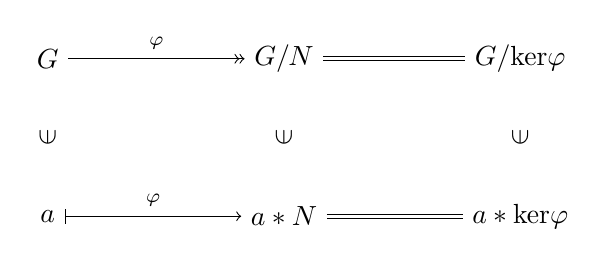
\begin{tikzpicture}[auto]
    \node[rotate=90] (a) at (0, 1) {$\in $};
    \node[rotate=90] (b) at (3, 1) {$\in $};
    \node[rotate=90] (c) at (6, 1) {$\in $};
    \node (a) at (0, 2) {$G$};
    \node (b) at (3, 2) {$G/N$};
    \node (c) at (6, 2) {$G/{\rm ker} \varphi $};
    \draw [->>] (a) to node {$\scriptstyle \varphi $} (b);
    \draw [double distance=1pt] (b) to node {$\scriptstyle $} (c);
    \node (a) at (0, 0) {$a$};
    \node (b) at (3, 0) {$a*N$};
    \node (c) at (6, 0) {$a*{\rm ker} \varphi $};
    \draw [|->] (a) to node {$\scriptstyle \varphi $} (b);
    \draw [double distance=1pt] (b) to node {$\scriptstyle $} (c);
  \end{tikzpicture}
\end{center}
\end{dfn}
\begin{proof}
群$(G,*)$の正規部分群$(N,*)$が与えられたとき、写像$\varphi:G \rightarrow G/N;a \mapsto a*N$について、$\forall a,b \in G$に対し、次のようになる。
\begin{align*}
\varphi(a*b) &= (a*b)*N\\
&= (a*b)*(N*N)\\
&= N*(a*b)*N\\
&= (a*N)*(b*N)\\
&= \varphi(a)*\varphi(b)
\end{align*}
これにより、その写像$\varphi$は群準同型写像である。\par
また、$\forall a*N$に対し、次のようになることから、
\begin{align*}
(a*N)*\left( 1_{(G,*)}*N \right) &= \varphi(a)*\varphi\left( 1_{(G,*)} \right)\\
&= \varphi\left( a*1_{(G,*)} \right)\\
&= \varphi(a) = a*N\\
&\left( 1_{(G,*)}*N \right)*(a*N) = \varphi\left( 1_{(G,*)} \right)*\varphi(a)\\
&= \varphi\left( 1_{(G,*)}*a \right)\\
&= \varphi(a) = a*N
\end{align*}
その群$(G/N,*)$の単位元は$1_{(G,*)}*N$である。したがって、$\forall a \in \ker\varphi$に対し、次のようになる。
\begin{align*}
\varphi(a) &= a*N\\
&= 1_{(G,*)}*N\\
&= N
\end{align*}
ここで、$\forall n \in N$に対し、$n = a*n'$なる元$n'$がその集合$N$に存在し次のようになるので、
\begin{align*}
a &= a*1_{(G,*)}\\
&= a*n'*{n'}^{- 1}\\
&= n*{n'}^{- 1} \in N
\end{align*}
$a \in N$が成り立つ。逆に、$\forall a \in N$が成り立つなら、次のようになるので、
\begin{align*}
\varphi(a) &= a*N\\
&= \left\{ a*n \in G \middle| n \in N \right\}\\
&= \left\{ a*n \in G \middle| a*n \in N \right\}\\
&= N
\end{align*}
$a \in \ker\varphi$が成り立つ。以上より、$\ker\varphi = N$が得られる。\par
最後に、$\forall a*N \in {G}/{N}$に対し、商群の定義より明らかに$\varphi(a) = a*N$なるその集合$G$の元$a$が存在するので、その写像$\varphi$は全射である。これにより、その写像$\varphi$は全射群準同型写像である。
\end{proof}
%\hypertarget{ux7fa4ux6e96ux540cux578bux5b9aux7406}{%
\subsubsection{群準同型定理}%\label{ux7fa4ux6e96ux540cux578bux5b9aux7406}}
\begin{thm}\label{3.1.2.8}
2つの群々$\left( G,*_{G} \right)$、$\left( H,*_{H} \right)$の間の群準同型写像$f:G \rightarrow H$について、$\forall a,b \in G$に対し、$f(a) = f(b)$が成り立つならそのときに限り、その群$\left( G,*_{G} \right)$の正規部分群$\left( \ker f,*_{G} \right)$を法としてその集合$G$の元々$a$、$b$が合同である、即ち、$a \equiv b\ \mathrm{mod}\left( \ker f,*_{G} \right)$が成り立つ。
\end{thm}
\begin{proof}
2つの群々$\left( G,*_{G} \right)$、$\left( H,*_{H} \right)$の間の群準同型写像$f:G \rightarrow H$について、$\forall a,b \in G$に対し、$f(a) = f(b)$が成り立つなら、その群準同型写像$f$の核$\ker f$を用いた組$\left( \ker f,*_{G} \right)$は定理\ref{3.1.2.6}よりその群$\left( G,*_{G} \right)$の正規部分群であり群準同型写像と核の定義より次のようになるので、
\begin{align*}
f\left( a^{- 1}*_{G}b \right) &= f\left( a^{- 1} \right)*_{H}f(b)\\
&= {f(a)}^{- 1}*_{H}f(b)\\
&= {f(b)}^{- 1}*_{H}f(b)\\
&= 1_{\left( H,*_{H} \right)}
\end{align*}
$a^{- 1}*_{G}b \in \ker f$が得られる。定理\ref{3.1.1.20}よりその正規部分群$\left( \ker f,*_{G} \right)$を法としてその集合$G$の元々$a$、$b$が合同である、即ち、$a \equiv b\ \mathrm{mod}\left( \ker f,*_{G} \right)$が成り立つ。
\end{proof}
\begin{thm}\label{3.1.2.9}
これの系として、2つの群々$\left( G,*_{G} \right)$、$\left( H,*_{H} \right)$の間の群準同型写像$f:G \rightarrow H$が単射であるならそのときに限り、その写像$f$の核$\ker f$が$\ker f = \left\{ 1_{\left( G,*_{G} \right)} \right\}$を満たす。
\end{thm}
\begin{proof}
2つの群々$\left( G,*_{G} \right)$、$\left( H,*_{H} \right)$の間の群準同型写像$f:G \rightarrow H$について、その群$\left( \left\{ 1_{\left( G,*_{G} \right)} \right\},*_{G} \right)$は、$1_{\left( G,*_{G} \right)} \in \left\{ 1_{\left( G,*_{G} \right)} \right\}$が成り立つかつ、$1_{\left( G,*_{G} \right)}*_{G}1_{\left( G,*_{G} \right)} \in \left\{ 1_{\left( G,*_{G} \right)} \right\}$が成り立つかつ、次のようになることから、
\begin{align*}
1_{\left( G,*_{G} \right)}^{- 1} &= 1_{\left( G,*_{G} \right)}^{- 1}*_{G}1_{\left( G,*_{G} \right)}\\
&= 1_{\left( G,*_{G} \right)}
\end{align*}
$1_{\left( G,*_{G} \right)}^{- 1} \in \left\{ 1_{\left( G,*_{G} \right)} \right\}$が成り立つので、定理\ref{3.1.1.6}よりその群$\left( G,*_{G} \right)$の部分群で、$\forall a \in G$に対し、次のようになるので、
\begin{align*}
1_{\left( G,*_{G} \right)} &= a*_{G}a^{- 1}\\
&= a*_{G}1_{\left( G,*_{G} \right)}*_{G}a^{- 1} \in \left\{ 1_{\left( G,*_{G} \right)} \right\}
\end{align*}
定理\ref{3.1.1.25}よりその群$\left( \left\{ 1_{\left( G,*_{G} \right)} \right\},*_{G} \right) \trianglelefteq \left( G,*_{G} \right)$が成り立つ。\par
その写像$f$の核$\ker f$が$\ker f = \left\{ 1_{\left( G,*_{G} \right)} \right\}$を満たすとき、2つの群々$\left( G,*_{G} \right)$、$\left( H,*_{H} \right)$の間の群準同型写像$f:G \rightarrow H$について、定理\ref{3.1.2.8}より次のようになる。
\begin{align*}
f(a) = f(b) &\Leftrightarrow a \equiv b\ \left( \mathrm{mod}\left\{ 1_{\left( G,*_{G} \right)} \right\} \right)\\
&\Leftrightarrow a^{- 1}*_{G}b \in \left\{ 1_{\left( G,*_{G} \right)} \right\}\\
&\Leftrightarrow a^{- 1}*_{G}b = 1_{\left( G,*_{G} \right)}\\
&\Leftrightarrow a*_{G}a^{- 1}*_{G}b = a*_{G}1_{\left( G,*_{G} \right)}\\
&\Leftrightarrow 1_{\left( G,*_{G} \right)}*_{G}b = a*_{G}1_{\left( G,*_{G} \right)}\\
&\Leftrightarrow a = b
\end{align*}
これにより、その写像$f$は単射である。\par
逆に、その写像$f$が単射であるなら、$\forall a,b \in G$に対し、次のようになる。
\begin{align*}
f(a) = f(b) &\Leftrightarrow a = b\\
&\Leftrightarrow a^{- 1}*_{G}a = a^{- 1}*_{G}b\\
&\Leftrightarrow a^{- 1}*_{G}b = 1_{\left( G,*_{G} \right)}\\
&\Leftrightarrow a^{- 1}*_{G}b \in \left\{ 1_{\left( G,*_{G} \right)} \right\}\\
&\Leftrightarrow a \equiv b\ \mathrm{mod}\left( \left\{ 1_{\left( G,*_{G} \right)} \right\},*_{G} \right)
\end{align*}
ここで、定理\ref{3.1.2.8}よりその写像$f$の核$\ker f$がその群$\left( G,*_{G} \right)$の単位元$1_{\left( G,*_{G} \right)}$のみからなる。
\end{proof}
\begin{thm}[群準同型定理]\label{3.1.2.10}
2つの群々$\left( G,*_{G} \right)$、$\left( H,*_{H} \right)$の間の群準同型写像$f:G \rightarrow H$について、写像$g:{G}/{\ker f} \rightarrow V(f);a*\ker f \mapsto f(a)$は群$\left( G/\ker f,*_{G} \right)$から群$\left( V(f),*_{H} \right)$への群同型写像でありこれらの2つの群々$\left( G/\ker f,*_{G} \right)$、$\left( V(f),*_{H} \right)$は群同型である、即ち、$\left( {G}/{\ker f},*_{G} \right) \cong \left( V(f),*_{H} \right)$が成り立つ。\par
この定理を群準同型定理という。この定理は、その群$\left( G,*_{G} \right)$からその商群$\left( {G}/{\ker f},*_{G} \right)$への自然な全射群準同型写像$\varphi$が用いられれば、次のように与えられる。
\begin{center}
  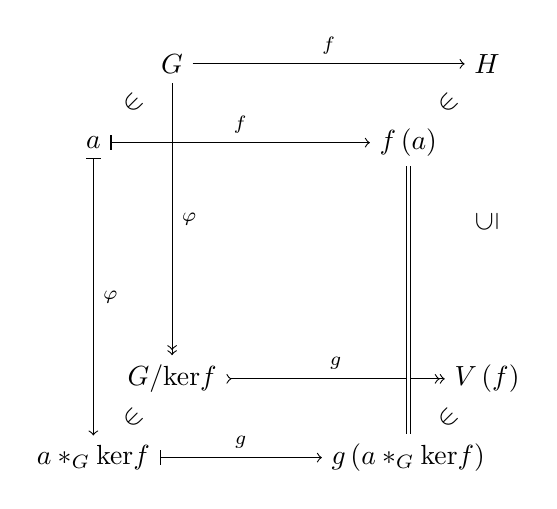
\begin{tikzpicture}[auto]
    \node (a) at (0, 0) {$a*_G {\rm ker} f$};
    \node (b) at (4, 0) {$g\left( a*_G {\rm ker} f\right) $};
    \node (c) at (0, 4) {$a$};
    \node (d) at (4, 4) {$f\left( a\right) $};
    \node (e) at (1, 1) {$G/{\rm ker} f$};
    \node (f) at (5, 1) {$V\left( f\right) $};
    \node (g) at (1, 5) {$G$};
    \node (h) at (5, 5) {$H$};
    \node[rotate=45] (i) at (0.5, 0.5) {$\in $};
    \node[rotate=45] (j) at (4.5, 0.5) {$\in $};
    \node[rotate=45] (k) at (0.5, 4.5) {$\in $};
    \node[rotate=45] (l) at (4.5, 4.5) {$\in $};
    \node[rotate=90] (m) at (5, 3) {$\subseteq $};
    \draw [|->] (a) to node {$\scriptstyle g$} (b);
    \draw [>->>] (e) to node {$\scriptstyle g$} (f);
    \draw [|->] (c) to node {$\scriptstyle \varphi $} (a);
    \draw [->>] (g) to node {$\scriptstyle \varphi $} (e);
    \draw [|->] (c) to node {$\scriptstyle f$} (d);
    \draw [->] (g) to node {$\scriptstyle f$} (h);
    \draw [double distance=1pt] (b) to node {$ $} (d);
  \end{tikzpicture} 
\end{center}
\end{thm}
\begin{proof}
2つの群々$\left( G,*_{G} \right)$、$\left( H,*_{H} \right)$の間の群準同型写像$f:G \rightarrow H$について、写像$g:{G}/{\ker f} \rightarrow V(f);a*_{G}\ker f \mapsto f(a)$が与えられるとき、$\forall a*_{G}\ker f,b*_{G}\ker f \in {G}/{\ker f}$に対し、$a*_{G}\ker f = b*_{G}\ker f$が成り立つなら、定理\ref{3.1.2.6}より$\left( \ker f,*_{G} \right) \trianglelefteq \left( G,*_{G} \right)$が成り立つので、$1_{\left( G,*_{G} \right)} \in \ker f$に注意すれば、$a*_{G}1_{\left( G,*_{G} \right)} \in a*_{G}\ker f = b*_{G}\ker f$が成り立つことにより、$\exists n \in \ker f$に対し、$a*_{G}1_{\left( G,*_{G} \right)} = b*_{G}n$が成り立つ。したがって、定理\ref{3.1.1.25}より次のようになる。
\begin{align*}
a*_{G}b^{- 1} &= a*_{G}1_{\left( G,*_{G} \right)}*_{G}b^{- 1}\\
&= b*_{G}n*_{G}b^{- 1} \in b*_{G}\ker f*_{G}b^{- 1} = \ker f
\end{align*}
ゆえに、次のようになる。
\begin{align*}
g\left( a*_{G}\ker f \right) &= f(a)\\
&= f(a)*_{H}1_{\left( H,*_{H} \right)}\\
&= f(a)*_{H}{f(b)}^{- 1}*_{H}f(b)\\
&= f(a)*_{H}f\left( b^{- 1} \right)*_{H}f(b)\\
&= f\left( a*_{G}b^{- 1} \right)*_{H}f(b)\\
&= 1_{\left( H,*_{H} \right)}*_{H}f(b)\\
&= f(b)\\
&= g\left( b*_{G}\ker f \right)
\end{align*}
ゆえに、その対応$g$は写像となっている。\par
その値域の定義より明らかにその写像$g$は全射である。また、$g\left( a*_{G}\ker f \right) = g\left( b*_{G}\ker f \right)$が成り立つなら、群$\left( \ker f,*_{G} \right)$はその群$\left( G,*_{G} \right)$の部分群であることにより次のようになる。
\begin{align*}
&\quad g\left( a*_{G}\ker f \right) = g\left( b*_{G}\ker f \right) \\
&\Leftrightarrow f(a) = f(b)\\
&\Leftrightarrow f(a)*_{H}{f(b)}^{- 1} = f(a)*_{H}f\left( b^{- 1} \right) = f\left( a*_{G}b^{- 1} \right) = 1_{\left( H,*_{H} \right)}\\
&\Leftrightarrow a*_{G}b^{- 1} \in \ker f\\
&\Leftrightarrow \left( a*_{G}b^{- 1} \right)^{- 1} = a^{- 1}*_{G}b \in \ker f
\end{align*}
ここで、定理\ref{3.1.1.18}よりその群$\left( G,*_{G} \right)$の部分群$\left( \ker f,*_{G} \right)$について、$a^{- 1}*_{G}b \in \ker f$が成り立つなら、$a*_{G}\ker f = b*_{G}\ker f$が成り立つのであったので、次のようになる。
\begin{align*}
g\left( a*_{G}\ker f \right) = g\left( b*_{G}\ker f \right) &\Leftrightarrow a^{- 1}*_{G}b \in \ker f\\
&\Rightarrow a*_{G}\ker f = b*_{G}\ker f
\end{align*}
したがって、その写像$g$は単射である。以上より、その写像$g$は全単射$g:{G}/{\ker f}\overset{\sim}{\rightarrow}V(f)$である。\par
その組$\left( \ker f,*_{G} \right)$はその群$\left( G,*_{G} \right)$の正規部分群であったので、$\forall a*_{G}\ker f,b*_{G}\ker f \in {G}/{\ker f}$に対し、次のようになる。
\begin{align*}
g\left( \left( a*_{G}\ker f \right)*_{G}\left( b*_{G}\ker f \right) \right) &= g\left( \ker f*_{G}a*_{G}b*_{G}\ker f \right)\\
&= g\left( \ker f*_{G}\left( a*_{G}b \right)*_{G}\ker f \right)\\
&= g\left( \left( a*_{G}b \right)*_{G}\ker f*_{G}\ker f \right)\\
&= g\left( \left( a*_{G}b \right)*_{G}\ker f \right)\\
&= f\left( a*_{G}b \right)\\
&= f(a)*_{H}f(b)\\
&= g\left( a*_{G}\ker f \right)*_{H}g\left( b*_{G}\ker f \right)
\end{align*}
これにより、その写像$g$は群準同型写像であり、その写像$g$は全単射だったので、その写像$g$は群同型写像である。\par
これにより、2つのそれらの群々$\left( G/\ker f,*_{G} \right)$、$\left( V(f),*_{H} \right)$は、その集合$G/\ker f$からその集合$V(f)$への群同型写像$g:{G}/{\ker f} \rightarrow V(f)$が存在するので、群同型である、即ち、$\left( {G}/{\ker f},*_{G} \right) \cong \left( V(f),*_{H} \right)$が成り立つ。\par
よって、その群$\left( G,*_{G} \right)$からその商群$\left( {G}/{\ker f},*_{G} \right)$への自然な全射群準同型写像$\varphi$が用いられれば、次のように与えられる。
\begin{center}
  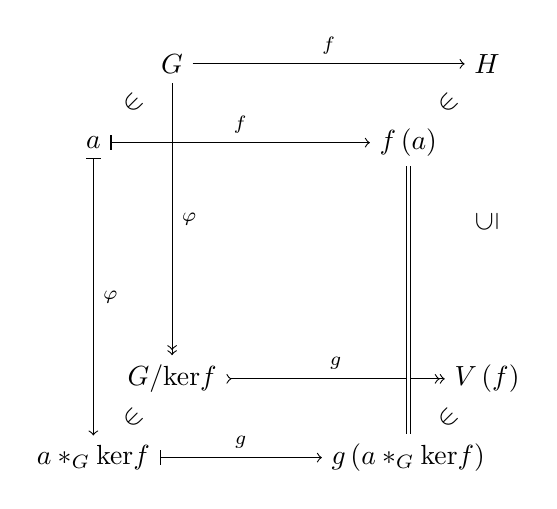
\begin{tikzpicture}[auto]
    \node (a) at (0, 0) {$a*_G {\rm ker} f$};
    \node (b) at (4, 0) {$g\left( a*_G {\rm ker} f\right) $};
    \node (c) at (0, 4) {$a$};
    \node (d) at (4, 4) {$f\left( a\right) $};
    \node (e) at (1, 1) {$G/{\rm ker} f$};
    \node (f) at (5, 1) {$V\left( f\right) $};
    \node (g) at (1, 5) {$G$};
    \node (h) at (5, 5) {$H$};
    \node[rotate=45] (i) at (0.5, 0.5) {$\in $};
    \node[rotate=45] (j) at (4.5, 0.5) {$\in $};
    \node[rotate=45] (k) at (0.5, 4.5) {$\in $};
    \node[rotate=45] (l) at (4.5, 4.5) {$\in $};
    \node[rotate=90] (m) at (5, 3) {$\subseteq $};
    \draw [|->] (a) to node {$\scriptstyle g$} (b);
    \draw [>->>] (e) to node {$\scriptstyle g$} (f);
    \draw [|->] (c) to node {$\scriptstyle \varphi $} (a);
    \draw [->>] (g) to node {$\scriptstyle \varphi $} (e);
    \draw [|->] (c) to node {$\scriptstyle f$} (d);
    \draw [->] (g) to node {$\scriptstyle f$} (h);
    \draw [double distance=1pt] (b) to node {$ $} (d);
  \end{tikzpicture} 
\end{center}
\end{proof}
\begin{dfn}
2つの群々$\left( G,*_{G} \right)$、$\left( H,*_{H} \right)$の間のある全射群準同型写像$f:G \twoheadrightarrow H$が存在するとき、その群$\left( H,*_{H} \right)$はその群$\left( G,*_{G} \right)$の群準同型像という。
\end{dfn}
\begin{thm}\label{3.1.2.11}
群$\left( H,*_{H} \right)$が群$\left( G,*_{G} \right)$の群準同型像であるならそのときに限り、その群$\left( H,*_{H} \right)$と群同型であるようなその群$\left( G,*_{G} \right)$のある商群が存在する。
\end{thm}
\begin{proof}
定義より群$\left( H,*_{H} \right)$が群$\left( G,*_{G} \right)$の群準同型像であるならそのときに限り、それらの群々$\left( G,*_{G} \right)$、$\left( H,*_{H} \right)$の間の全射群準同型写像$f:G \twoheadrightarrow H$が存在するのであった。このとき、群準同型定理と$V(f) = H$が成り立つことより写像$g:G/\ker f\overset{\sim}{\rightarrow}H$は群同型写像でありそれらの群々$\left( {G}/{\ker f},*_{G} \right)$、$\left( H,*_{H} \right)$は群同型である。したがって、その群$\left( H,*_{H} \right)$と群同型であるようなその群$\left( G,*_{G} \right)$のある商群が存在する。\par
逆に、その群$\left( H,*_{H} \right)$と群同型であるようなその群$\left( G,*_{G} \right)$のある商群が存在するなら、その群$\left( G,*_{G} \right)$のある正規部分群$\left( N,*_{G} \right)$を用いてその商群が$\left( {G}/{N},*_{G} \right)$とおかれれば、群同型写像$g:{G}/{N}\overset{\sim}{\rightarrow}H$が存在できる。また、写像$\varphi:G \rightarrow {G}/{N};a \mapsto a*_{G}N$は定理\ref{3.1.2.7}より全射群準同型写像で$\ker\varphi = N$が成り立つのであったので、次式のような写像$g \circ \varphi$を考えると、
\begin{center}
  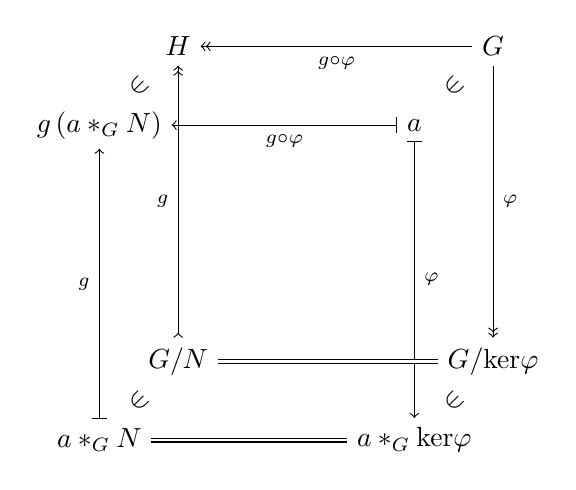
\begin{tikzpicture}[auto]
    \node[rotate=45] (x) at (7.5, 0.5) {$\in $};
    \node[rotate=45] (x) at (7.5, 4.5) {$\in $};
    \node[rotate=45] (x) at (3.5, 0.5) {$\in $};
    \node[rotate=45] (x) at (3.5, 4.5) {$\in $};
    \node (a) at (7, 0) {$a*_G {\rm ker} \varphi $};
    \node (c) at (7, 4) {$a$};
    \node (e) at (8, 1) {$G/{\rm ker} \varphi $};
    \node (g) at (8, 5) {$G$};
    \node (i) at (3, 0) {$a*_G N$};
    \node (j) at (3, 4) {$g\left( a*_G N\right) $};
    \node (k) at (4, 1) {$G/N$};
    \node (l) at (4, 5) {$H$};
    \draw [|->] (c) to node {$\scriptstyle \varphi $} (a);
    \draw [->>] (g) to node {$\scriptstyle \varphi $} (e);
    \draw [double distance=1pt] (a) to node {} (i);
    \draw [double distance=1pt] (e) to node {} (k);
    \draw [|->] (i) to node {$\scriptstyle g$} (j);
    \draw [>->>] (k) to node {$\scriptstyle g$} (l);
    \draw [|->] (c) to node {$\scriptstyle g\circ \varphi $} (j);
    \draw [->>] (g) to node {$\scriptstyle g\circ \varphi $} (l);
  \end{tikzpicture} 
\end{center}
これは全射群準同型写像$g \circ \varphi:G \twoheadrightarrow H$であるので、その群$\left( H,*_{H} \right)$はその群$\left( G,*_{G} \right)$の群準同型像である。
\end{proof}
%\hypertarget{ux7fa4ux540cux578bux5b9aux7406}{%
\subsubsection{群同型定理}%\label{ux7fa4ux540cux578bux5b9aux7406}}
\begin{thm}\label{3.1.2.12}
2つの群々$\left( G,*_{G} \right)$、$\left( H,*_{H} \right)$の間の全射群準同型写像$f:G \twoheadrightarrow H$について、その群$\left( G,*_{G} \right)$の部分群$\left( I,*_{G} \right)$と正規部分群$\left( M,*_{G} \right)$を用いた2つの組々$\left( V\left( f|I \right),*_{H} \right)$、$\left( V\left( f|M \right),*_{H} \right)$はそれぞれその群$\left( H,*_{H} \right)$の部分群、正規部分群である。\par
また、その群$\left( H,*_{H} \right)$の部分群$\left( J,*_{H} \right)$と正規部分群$\left( N,*_{H} \right)$を用いた2つの組々$\left( V\left( f^{- 1}|J \right),*_{G} \right)$、$\left( V\left( f^{- 1}|N \right),*_{G} \right)$はそれぞれその群$\left( G,*_{G} \right)$の部分群、正規部分群である。
\end{thm}
\begin{proof}
2つの群々$\left( G,*_{G} \right)$、$\left( H,*_{H} \right)$の間の全射群準同型写像$f:G \twoheadrightarrow H$について、その群$\left( G,*_{G} \right)$の部分群$\left( I,*_{G} \right)$と正規部分群$\left( M,*_{G} \right)$を用いた2つの組々$\left( V\left( f|I \right),*_{H} \right)$、$\left( V\left( f|M \right),*_{H} \right)$が与えられたとする。$f|I(a),f|I(b) \in V\left( f|I \right)$のとき、定理\ref{3.1.1.6}より$a,b \in I$が成り立つなら、$a*_{G}b \in I$も成り立つので、次のようになる。
\begin{align*}
f|I(a)*_{H}f|I(b) = f|I\left( a*_{G}b \right) \in V\left( f|I \right)
\end{align*}
$f|I\left( a^{- 1} \right) = {f|I(a)}^{- 1}$が成り立つことと定理\ref{3.1.1.6}より$a \in I$が成り立つなら、$a^{- 1} \in I$も成り立つので、次のようになる。
\begin{align*}
{f|I(a)}^{- 1} = f|I\left( a^{- 1} \right) \in V\left( f|I \right)
\end{align*}
したがって、組$\left( V\left( f|I \right),*_{H} \right)$は定理\ref{3.1.1.6}よりその群$\left( H,*_{H} \right)$の部分群である。\par
同様にして、群$\left( V\left( f|M \right),*_{H} \right)$はその群$\left( H,*_{H} \right)$の部分群であることが示され、$f|M\left( a^{- 1} \right) =$
${f|M(a)}^{- 1}$が成り立つことと定理\ref{3.1.1.25}より$h \in M$が成り立つなら、$\forall b \in G$に対し、$b*_{G}h*_{G}b^{- 1} \in M$も成り立つので、次のようになる。
\begin{align*}
f(b)*_{H}f|M(a)*_{H}{f(b)}^{- 1} &= f(b)*_{H}f(a)*_{H}f\left( b^{- 1} \right)\\
&= f\left( b*_{G}h*_{G}b^{- 1} \right) \in V\left( f|M \right)
\end{align*}
したがって、組$\left( V\left( f|M \right),*_{H} \right)$は定理\ref{3.1.1.25}よりその群$\left( H,*_{H} \right)$の正規部分群である。\par
また、その群$\left( H,*_{H} \right)$の部分群$\left( J,*_{H} \right)$と正規部分群$\left( N,*_{H} \right)$を用いた2つの集合たち$V\left( f^{- 1}|J \right)$、$V\left( f^{- 1}|N \right)$が与えられたとする。群準同型写像の定義と定理\ref{3.1.1.6}より$a,b \in J$が成り立つなら、$a*_{H}b \in J$も成り立つので、次のようになる。
\begin{align*}
a,b \in V\left( f^{- 1}|J \right) &\Rightarrow f(a),f(b) \in V\left( f|V\left( f^{- 1}|J \right) \right) \subseteq J\\
&\Rightarrow f(a)*_{H}f(b) = f\left( a*_{H}b \right) \in J\\
&\Rightarrow a*_{G}b \in V\left( f^{- 1}|J \right)
\end{align*}
$f\left( a^{- 1} \right) = {f(a)}^{- 1}$が成り立つことと定理\ref{3.1.1.6}より$a \in J$が成り立つなら、$a^{- 1} \in J$も成り立つので、次のようになる。
\begin{align*}
a \in V\left( f^{- 1}|J \right) &\Rightarrow f(a) \in V\left( f|V\left( f^{- 1}|J \right) \right) \subseteq J\\
&\Rightarrow {f(a)}^{- 1} = f\left( a^{- 1} \right) \in J\\
&\Rightarrow a^{- 1} \in V\left( f^{- 1}|J \right)
\end{align*}
したがって、組$\left( V\left( f^{- 1}|J \right),*_{G} \right)$はその群$\left( G,*_{G} \right)$の部分群である。\par
同様にして、組$\left( V\left( f^{- 1}|N \right),*_{G} \right)$はその群$\left( G,*_{G} \right)$の部分群であることが示され群準同型写像の定義と${f(a)}^{- 1} = f\left( a^{- 1} \right)$が成り立つことと正規部分群の定義より次のようになる。
\begin{align*}
b \in a*_{G}V\left( f^{- 1}|N \right) &\Leftrightarrow a^{- 1}*_{G}b \in a^{- 1}*_{G}a*_{G}V\left( f^{- 1}|N \right) = 1_{\left( G,*_{G} \right)}*_{G}V\left( f^{- 1}|N \right) = V\left( f^{- 1}|N \right)\\
&\Leftrightarrow f\left( a^{- 1}*_{G}b \right) \in V\left( f|V\left( f^{- 1}|N \right) \right) \subseteq N\\
&\Rightarrow f\left( a^{- 1} \right)*_{H}f(b) = {f(a)}^{- 1}*_{H}f(b) \in N\\
&\Leftrightarrow f(a)*_{H}{f(a)}^{- 1}*_{H}f(b) = 1_{\left( H,*_{H} \right)}*_{H}f(b) = f(b) \in f(a)*_{H}N\\
&\Leftrightarrow f(b) \in f(a)*_{H}N = N*_{H}f(a)\\
&\Leftrightarrow f(b)*_{H}{f(a)}^{- 1} \in N*_{H}f(a)*_{H}{f(a)}^{- 1} = N*_{H}1_{\left( H,*_{H} \right)} = N\\
&\Leftrightarrow f(b)*_{H}{f(a)}^{- 1} = f(b)*_{H}f\left( a^{- 1} \right) = f\left( b*_{G}a^{- 1} \right) \in N\\
&\Leftrightarrow b*_{G}a^{- 1} \in V\left( f^{- 1}|N \right)\\
&\Leftrightarrow b*_{G}a^{- 1}*_{G}a = b*_{G}1_{\left( G,*_{G} \right)} = b \in V\left( f^{- 1}|N \right)*_{G}a
\end{align*}
これにより、$a*_{G}V\left( f^{- 1}|N \right) \subseteq V\left( f^{- 1}|N \right)*_{G}a$が成り立つ。同様にして、$a*_{G}V\left( f^{- 1}|N \right) \supseteq V\left( f^{- 1}|N \right)*_{G}a$も成り立つことが示されるので、$a*_{G}V\left( f^{- 1}|N \right) = V\left( f^{- 1}|N \right)*_{G}a$が成り立ち、したがって、組$\left( V\left( f^{- 1}|N \right),*_{G} \right)$はその群$\left( G,*_{G} \right)$の正規部分群である。
\end{proof}
\begin{thm}[第1群同型定理]\label{3.1.2.13}
2つの群々$\left( G,*_{G} \right)$、$\left( H,*_{H} \right)$の間の全射群準同型写像$f:G \twoheadrightarrow H$について、その群$\left( G,*_{G} \right)$の部分群をなす$\ker f \subseteq I$が成り立つようなその集合$G$の部分集合全体の集合を$\varOmega_{\left( G,*_{G} \right)}'$、その群$\left( H,*_{H} \right)$の部分群をなすその集合$H$の部分集合全体の集合を$\varOmega_{\left( H,*_{H} \right)}$とおくと、次のことが成り立つ。
\begin{itemize}
\item
  次式のように写像$F:\varOmega_{\left( G,*_{G} \right)}' \rightarrow \varOmega_{\left( H,*_{H} \right)};I \mapsto V\left( f|I \right)$は全単射でその逆写像$F^{- 1}$が$F^{- 1}:\varOmega_{\left( H,*_{H} \right)} \rightarrow \varOmega_{\left( G,*_{G} \right)}';J \mapsto V\left( f^{- 1}|J \right)$と与えられる。
  \begin{center}
    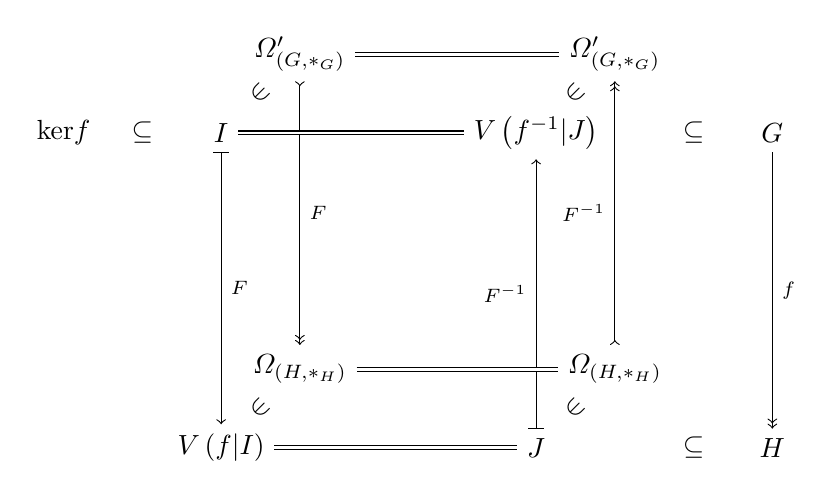
\begin{tikzpicture}[auto]
      \node[rotate=45] (x) at (2.5, 4.5) {$\in $};
      \node[rotate=45] (x) at (2.5, 0.5) {$\in $};
      \node[rotate=45] (x) at (6.5, 0.5) {$\in $};
      \node[rotate=45] (x) at (6.5, 4.5) {$\in $};
      \node (y) at (1, 4) {$\subseteq $};
      \node (y) at (8, 4) {$\subseteq $};
      \node (y) at (8, 0) {$\subseteq $};
      \node (a) at (3, 5) {$\varOmega_{\left(G,*_G \right)}' $};
      \node (b) at (3, 1) {$\varOmega_{\left(H,*_H \right)} $};
      \node (c) at (2, 4) {$I$};
      \node (d) at (2, 0) {$V\left( f|I\right) $};
      \node (e) at (6, 0) {$J$};
      \node (f) at (6, 4) {$V\left( f^{-1} |J\right) $};
      \node (g) at (7, 1) {$\varOmega_{\left(H,*_H \right)} $};
      \node (h) at (7, 5) {$\varOmega_{\left(G,*_G \right)}' $};
      \node (i) at (9, 4) {$G$};
      \node (j) at (9, 0) {$H$};
      \node (k) at (0, 4) {${\rm ker} f$};
      \draw [>->>] (a) to node {$\scriptstyle F$} (b);
      \draw [|->] (c) to node {$\scriptstyle F$} (d);
      \draw [>->>] (g) to node {$\scriptstyle F^{-1} $} (h);
      \draw [|->] (e) to node {$\scriptstyle F^{-1} $} (f);
      \draw [->>] (i) to node {$\scriptstyle f$} (j);
      \draw [double distance=1pt] (c) to node {} (f);
      \draw [double distance=1pt] (d) to node {} (e);
      \draw [double distance=1pt] (a) to node {} (h);
      \draw [double distance=1pt] (b) to node {} (g);
    \end{tikzpicture} 
  \end{center}
\item
  $\forall I \in \varOmega_{\left( G,*_{G} \right)}'$に対し、$\left( {I}/{\ker f},*_{G} \right) \cong \left( F(I),*_{H} \right)$が成り立つ。これは次式のようにも表される。
  \begin{center}
    \begin{tikzpicture}[auto]
      \node[rotate=45] (x) at (2.5, 4.5) {$\in $};
      \node[rotate=45] (x) at (2.5, 0.5) {$\in $};
      \node (y) at (1, 4) {$\subseteq $};
      \node (y) at (7, 4) {$\subseteq $};
      \node (y) at (7, 0) {$\subseteq $};
      \node (a) at (3, 5) {$\varOmega_{\left(G,*_G \right)}' $};
      \node (b) at (3, 1) {$\varOmega_{\left(H,*_H \right)} $};
      \node (c) at (2, 4) {$I$};
      \node (d) at (2, 0) {$V\left( f|I\right) $};
      \node (e) at (6, 0) {$J$};
      \node (f) at (12, 4) {$I/{\rm ker} f$};
      \node (i) at (8, 4) {$G$};
      \node (j) at (8, 0) {$H$};
      \node (k) at (0, 4) {${\rm ker} f$};
      \draw [>->>] (a) to node {$\scriptstyle F$} (b);
      \draw [|->] (c) to node {$\scriptstyle F$} (d);
      \draw [>->>] (f) to node {} (e);
      \draw [->>] (i) to node {$\scriptstyle f$} (j);
      \draw [double distance=1pt] (d) to node {} (e);
      \draw [->>] (c)[bend left=10] to node {} (f);
    \end{tikzpicture} 
  \end{center}
\end{itemize}
\begin{itemize}
\item
  $\forall I \in \varOmega_{\left( G,*_{G} \right)}'$に対し、その写像$F:\varOmega_{\left( G,*_{G} \right)}' \rightarrow \varOmega_{\left( H,*_{H} \right)};I \mapsto V\left( f|I \right)$が与えられたとき、$\left( I,*_{G} \right) \trianglelefteq \left( G,*_{G} \right)$が成り立つならそのときに限り、$\left( F(I),*_{H} \right) \trianglelefteq \left( H,*_{H} \right)$が成り立つ。
\item
  $\forall I \in \varOmega_{\left( G,*_{G} \right)}'$に対し、上記の写像$F:\varOmega_{\left( G,*_{G} \right)}' \rightarrow \varOmega_{\left( H,*_{H} \right)};I \mapsto V\left( f|I \right)$が与えられたとき、$\left( I,*_{G} \right) \trianglelefteq \left( G,*_{G} \right)$が成り立つなら、$\left( G/I,*_{G} \right) \cong \left( H/F(I),*_{H} \right)$が成り立つ。これは次式のようにも表される。
  \begin{center}
    \begin{tikzpicture}[auto]
      \node[rotate=45] (x) at (2.5, 4.5) {$\in $};
      \node[rotate=45] (x) at (2.5, 0.5) {$\in $};
      \node (y) at (1, 4) {$\subseteq $};
      \node (y) at (7, 4) {$\subseteq $};
      \node (y) at (7, 0) {$\subseteq $};
      \node (a) at (3, 5) {$\varOmega_{\left(G,*_G \right)}' $};
      \node (b) at (3, 1) {$\varOmega_{\left(H,*_H \right)} $};
      \node (c) at (2, 4) {$I$};
      \node (d) at (2, 0) {$V\left( f|I\right) $};
      \node (e) at (6, 0) {$J$};
      \node (g) at (12, 0) {$H/J$};
      \node (h) at (12, 4) {$G/I$};
      \node (i) at (8, 4) {$G$};
      \node (j) at (8, 0) {$H$};
      \node (k) at (0, 4) {${\rm ker} f$};
      \draw [>->>] (a) to node {$\scriptstyle F$} (b);
      \draw [|->] (c) to node {$\scriptstyle F$} (d);
      \draw [>->>] (h) to node {} (g);
      \draw [->>] (i) to node {$\scriptstyle f$} (j);
      \draw [double distance=1pt] (d) to node {} (e);
      \draw [->>] (i) to node {} (h);
      \draw [->>] (j) to node {} (g);
    \end{tikzpicture} 
  \end{center}
\end{itemize}\par
この定理を第1群同型定理という。
\end{thm}
\begin{proof}
2つの群々$\left( G,*_{G} \right)$、$\left( H,*_{H} \right)$の間の全射群準同型写像$f:G \twoheadrightarrow H$について、その群$\left( G,*_{G} \right)$の部分群をなすその集合$G$のその核$\ker f$を含む部分集合全体の集合を$\varOmega_{\left( G,*_{G} \right)}'$、その群$\left( H,*_{H} \right)$の部分群をなすその集合$H$の部分集合全体の集合を$\varOmega_{\left( H,*_{H} \right)}$とおく。次式のように写像$F:\varOmega_{\left( G,*_{G} \right)}' \rightarrow \varOmega_{\left( H,*_{H} \right)};I \mapsto V\left( f|I \right) = J$を考えよう。
\begin{center}
  \begin{tikzpicture}[auto]
    \node[rotate=45] (x) at (2.5, 4.5) {$\in $};
    \node[rotate=45] (x) at (2.5, 0.5) {$\in $};
    \node (y) at (1, 4) {$\subseteq $};
    \node (y) at (7, 4) {$\subseteq $};
    \node (y) at (7, 0) {$\subseteq $};
    \node (a) at (3, 5) {$\varOmega_{\left(G,*_G \right)}' $};
    \node (b) at (3, 1) {$\varOmega_{\left(H,*_H \right)} $};
    \node (c) at (2, 4) {$I$};
    \node (d) at (2, 0) {$V\left( f|I\right) $};
    \node (e) at (6, 0) {$J$};
    \node (i) at (8, 4) {$G$};
    \node (j) at (8, 0) {$H$};
    \node (k) at (0, 4) {${\rm ker} f$};
    \draw [->] (a) to node {$\scriptstyle F$} (b);
    \draw [|->] (c) to node {$\scriptstyle F$} (d);
    \draw [->>] (i) to node {$\scriptstyle f$} (j);
    \draw [double distance=1pt] (d) to node {} (e);
  \end{tikzpicture} 
\end{center}
$\forall I \in \varOmega_{\left( G,*_{G} \right)}'$に対し、$V\left( f|I \right) = J$とおくと、定理\ref{3.1.2.12}よりその群$\left( G,*_{G} \right)$の部分群$\left( I,*_{G} \right)$を用いた組$\left( J,*_{H} \right)$はその群$\left( H,*_{H} \right)$の部分群であったので、$F(I) = V\left( f|I \right) \in \varOmega_{\left( H,*_{H} \right)}$が成り立つ。したがって、写像$F:\varOmega_{\left( G,*_{G} \right)}' \rightarrow \varOmega_{\left( H,*_{H} \right)};I \mapsto V\left( f|I \right)$が定義できている。ここで、次式のように写像$E:\varOmega_{\left( H,*_{H} \right)} \rightarrow \varOmega_{\left( G,*_{G} \right)}';J \mapsto V\left( f^{- 1}|J \right) = I$を考えよう。
\begin{center}
  \begin{tikzpicture}[auto]
    \node[rotate=45] (x) at (2.5, 4.5) {$\in $};
    \node[rotate=45] (x) at (2.5, 0.5) {$\in $};
    \node[rotate=45] (x) at (6.5, 0.5) {$\in $};
    \node[rotate=45] (x) at (6.5, 4.5) {$\in $};
    \node (y) at (1, 4) {$\subseteq $};
    \node (y) at (8, 4) {$\subseteq $};
    \node (y) at (8, 0) {$\subseteq $};
    \node (a) at (3, 5) {$\varOmega_{\left(G,*_G \right)}' $};
    \node (b) at (3, 1) {$\varOmega_{\left(H,*_H \right)} $};
    \node (c) at (2, 4) {$I$};
    \node (d) at (2, 0) {$V\left( f|I\right) $};
    \node (e) at (6, 0) {$J$};
    \node (f) at (6, 4) {$V\left( f^{-1} |J\right) $};
    \node (g) at (7, 1) {$\varOmega_{\left(H,*_H \right)} $};
    \node (h) at (7, 5) {$\varOmega_{\left(G,*_G \right)}' $};
    \node (i) at (9, 4) {$G$};
    \node (j) at (9, 0) {$H$};
    \node (k) at (0, 4) {${\rm ker} f$};
    \draw [->] (a) to node {$\scriptstyle F$} (b);
    \draw [|->] (c) to node {$\scriptstyle F$} (d);
    \draw [->] (g) to node {$\scriptstyle E$} (h);
    \draw [|->] (e) to node {$\scriptstyle E$} (f);
    \draw [->>] (i) to node {$\scriptstyle f$} (j);
    \draw [double distance=1pt] (d) to node {} (e);
    \draw [double distance=1pt] (a) to node {} (h);
    \draw [double distance=1pt] (b) to node {} (g);
  \end{tikzpicture} 
\end{center}
$\forall J \in \varOmega_{\left( H,*_{H} \right)}$に対し、$V\left( f^{- 1}|J \right) = I$とおくと、$\left\{ 1_{\left( H,*_{H} \right)} \right\} \subseteq J$が成り立つことから、$\ker f = V\left( f^{- 1}|\left\{ 1_{\left( H,*_{H} \right)} \right\} \right) \subseteq V\left( f^{- 1}|J \right) = I$が成り立つかつ、定理\ref{3.1.2.12}よりその群$\left( H,*_{H} \right)$の部分群$\left( J,*_{H} \right)$を用いた組$\left( I,*_{G} \right)$はその群$\left( G,*_{G} \right)$の部分群であったので、$E(J) = V\left( f^{- 1}|J \right) \in \varOmega_{\left( G,*_{G} \right)}'$が成り立つ。したがって、写像$E:\varOmega_{\left( H,*_{H} \right)} \rightarrow \varOmega_{\left( G,*_{G} \right)}';J \mapsto V\left( f^{- 1}|J \right)$が考えられることができる。\par
まず、$E \circ F = I_{\varOmega_{\left( G,*_{G} \right)}'}$が成り立つことを示そう。このとき、$\forall I \in \varOmega_{\left( G,*_{G} \right)}'$に対し、$V\left( f^{- 1}|V\left( f|I \right) \right) \supseteq I$は明らかに成り立つ。逆に、$\forall a \in G$に対し、$a \in V\left( f^{- 1}|V\left( f|I \right) \right)$が成り立つなら、$V\left( f|V\left( f^{- 1}|V\left( f|I \right) \right) \right) \subseteq V\left( f|I \right)$が成り立つので、$f(a) \in V\left( f|V\left( f^{- 1}|V\left( f|I \right) \right) \right) \subseteq V\left( f|I \right)$が成り立ち、したがって、$f(a) = f(b)$なるその集合$I$の元$b$が存在する。ここで、定理\ref{3.1.2.8}よりこれが成り立つならそのときに限り、$a \equiv b\ \mathrm{mod}\left( \ker f,*_{G} \right)$が成り立つのであったので、$a*_{G}b^{- 1} \in \ker f$が成り立ち、その集合$\varOmega_{\left( G,*_{G} \right)}'$の定義より、$a*_{G}b^{- 1} \in I$が成り立つ。したがって、$b \in I$が成り立つことと定理\ref{3.1.1.6}より次のようになる。
\begin{align*}
\left( a*_{G}b^{- 1} \right)*_{G}b &= a*_{G}\left( b^{- 1}*_{G}b \right)\\
&= a*_{G}1_{\left( G,*_{G} \right)}\\
&= a \in I
\end{align*}
以上より、$a \in I$が成り立つので、$V\left( f^{- 1}|V\left( f|I \right) \right) \subseteq I$が成り立つ。したがって、$V\left( f^{- 1}|V\left( f|I \right) \right) = I$が成り立つので、$E \circ F(I) = I$が成り立つ。\par
次に、$F \circ G = I_{\varOmega_{\left( H,*_{H} \right)}}$が成り立つことを示そう。$\forall J \in \varOmega_{\left( H,*_{H} \right)}$に対し、その対応$f$は写像なので、もちろん、$V\left( f|V\left( f^{- 1}|J \right) \right) = J$は成り立つ。したがって、$F \circ G(J) = V\left( f|V\left( f^{- 1}|J \right) \right) = J$が成り立つ。\par
以上より、$E \circ F = I_{\varOmega_{\left( G,*_{G} \right)}'}$かつ$F \circ G = I_{\varOmega_{\left( H,*_{H} \right)}}$が成り立つので、その写像$F:\varOmega_{\left( G,*_{G} \right)}' \rightarrow \varOmega_{\left( H,*_{H} \right)}$は全単射でその写像$E$がその写像$F$の逆写像である。よって、次式のように写像$F:\varOmega_{\left( G,*_{G} \right)}' \rightarrow \varOmega_{\left( H,*_{H} \right)};I \mapsto V\left( f|I \right)$は全単射でその逆写像$F^{- 1}$が$F^{- 1}:\varOmega_{\left( H,*_{H} \right)} \rightarrow \varOmega_{\left( G,*_{G} \right)}';J \mapsto V\left( f^{- 1}|J \right)$と与えられる。\par
また、$\forall I \in \varOmega_{\left( G,*_{G} \right)}'$に対し、$F(I) = V\left( f|I \right) = J$とおくと、写像$f':I \rightarrow J;a \mapsto f(a)$は明らかに全射群準同型写像であるから、次式のように考えられると、
\begin{center}
  \begin{tikzpicture}[auto]
    \node[rotate=45] (x) at (2.5, 4.5) {$\in $};
    \node[rotate=45] (x) at (2.5, 0.5) {$\in $};
    \node[rotate=45] (x) at (6.5, 4.5) {$\in $};
    \node (a) at (3, 5) {$I$};
    \node (b) at (3, 1) {$I/{\rm ker} f' $};
    \node (c) at (2, 4) {$a$};
    \node (d) at (2, 0) {$a*_G {\rm ker} f' $};
    \node (f) at (6, 4) {$f\left( a\right) $};
    \node (g) at (7, 1) {$V\left( f'|I\right) $};
    \node (h) at (7, 5) {$J$};
    \draw [->>] (a) to node {} (b);
    \draw [|->] (c) to node {} (d);
    \draw [->>] (a) to node {$\scriptstyle f'$} (h);
    \draw [|->] (c) to node {$\scriptstyle f'$} (f);
    \draw [double distance=1pt] (g) to node {} (h);
  \end{tikzpicture} 
\end{center}
群準同型定理より次式が成り立つので、
\begin{center}
  \begin{tikzpicture}[auto]
    \node[rotate=45] (x) at (2.5, 4.5) {$\in $};
    \node[rotate=45] (x) at (2.5, 0.5) {$\in $};
    \node[rotate=45] (x) at (6.5, 4.5) {$\in $};
    \node (a) at (3, 5) {$I$};
    \node (b) at (3, 1) {$I/{\rm ker} f' $};
    \node (c) at (2, 4) {$a$};
    \node (d) at (2, 0) {$a*_G {\rm ker} f' $};
    \node (f) at (6, 4) {$f\left( a\right) $};
    \node (g) at (7, 1) {$V\left( f'|I\right) $};
    \node (h) at (7, 5) {$J$};
    \draw [->>] (a) to node {} (b);
    \draw [|->] (c) to node {} (d);
    \draw [->>] (a) to node {$\scriptstyle f'$} (h);
    \draw [|->] (c) to node {$\scriptstyle f'$} (f);
    \draw [double distance=1pt] (g) to node {} (h);
    \draw [>->>] (b) to node {} (g);
  \end{tikzpicture} 
\end{center}
$\left( {I}/{\ker f'},*_{G} \right) \cong \left( V\left( f'|I \right),*_{H} \right)$が得られる。$\ker f \subseteq I$より$V\left( f'|I \right) = V\left( f|I \right) = J$が成り立つかつ、$\ker f' = \ker f$が成り立つので、$\left( {I}/{\ker f},*_{G} \right) \cong \left( J,*_{H} \right)$が成り立つ。\par
$\forall I \in \varOmega_{\left( G,*_{G} \right)}'$に対し、その写像$F:\varOmega_{\left( G,*_{G} \right)}' \rightarrow \varOmega_{\left( H,*_{H} \right)};I \mapsto V\left( f|I \right)$が与えられたとき、定理\ref{3.1.2.12}より$\left( I,*_{G} \right) \trianglelefteq \left( G,*_{G} \right)$が成り立つならそのときに限り、$\left( F(I),*_{H} \right) \trianglelefteq \left( H,*_{H} \right)$が成り立つことが直ちに分かる。\par
$\forall I \in \varOmega_{\left( G,*_{G} \right)}'$に対し、上記の写像$F:\varOmega_{\left( G,*_{G} \right)}' \rightarrow \varOmega_{\left( H,*_{H} \right)};I \mapsto V\left( f|I \right)$が与えられたとき、$\left( I,*_{G} \right) \trianglelefteq \left( G,*_{G} \right)$が成り立つなら、$F(I) = V\left( f|I \right) = J$とおいて次式のように自然な全射群準同型写像$\varphi_{H}:H \twoheadrightarrow H/J$を考えると、
\begin{center}
  \begin{tikzpicture}[auto]
    \node[rotate=45] (x) at (2.5, 4.5) {$\in $};
    \node[rotate=45] (x) at (2.5, 0.5) {$\in $};
    \node (y) at (1, 4) {$\subseteq $};
    \node (y) at (7, 4) {$\subseteq $};
    \node (y) at (7, 0) {$\subseteq $};
    \node (a) at (3, 5) {$\varOmega_{\left(G,*_G \right)}' $};
    \node (b) at (3, 1) {$\varOmega_{\left(H,*_H \right)} $};
    \node (c) at (2, 4) {$I$};
    \node (d) at (2, 0) {$V\left( f|I\right) $};
    \node (e) at (6, 0) {$J$};
    \node (g) at (12, 0) {$H/J$};
    \node (i) at (8, 4) {$G$};
    \node (j) at (8, 0) {$H$};
    \node (k) at (0, 4) {${\rm ker} f$};
    \draw [>->>] (a) to node {$\scriptstyle F$} (b);
    \draw [|->] (c) to node {$\scriptstyle F$} (d);
    \draw [->>] (i) to node {$\scriptstyle f$} (j);
    \draw [double distance=1pt] (d) to node {} (e);
    \draw [->>] (j) to node {$\scriptstyle \varphi_H $} (g);
  \end{tikzpicture} 
\end{center}
$J = \ker\varphi_{H}$が成り立ち、$\varphi_{H} \circ f = \rho$とおくと、その写像$\rho$は次式のように全射群準同型写像で、
\begin{center}
  \begin{tikzpicture}[auto]
    \node[rotate=45] (x) at (2.5, 4.5) {$\in $};
    \node[rotate=45] (x) at (2.5, 0.5) {$\in $};
    \node (y) at (1, 4) {$\subseteq $};
    \node (y) at (7, 4) {$\subseteq $};
    \node (y) at (7, 0) {$\subseteq $};
    \node (a) at (3, 5) {$\varOmega_{\left(G,*_G \right)}' $};
    \node (b) at (3, 1) {$\varOmega_{\left(H,*_H \right)} $};
    \node (c) at (2, 4) {$I$};
    \node (d) at (2, 0) {$V\left( f|I\right) $};
    \node (e) at (6, 0) {$J$};
    \node (g) at (12, 0) {$H/J$};
    \node (i) at (8, 4) {$G$};
    \node (j) at (8, 0) {$H$};
    \node (k) at (0, 4) {${\rm ker} f$};
    \draw [>->>] (a) to node {$\scriptstyle F$} (b);
    \draw [|->] (c) to node {$\scriptstyle F$} (d);
    \draw [->>] (i) to node {$\scriptstyle f$} (j);
    \draw [double distance=1pt] (d) to node {} (e);
    \draw [->>] (j) to node {$\scriptstyle \varphi_H $} (g);
    \draw [->>] (i) to node {$\scriptstyle \rho $} (g);
  \end{tikzpicture} 
\end{center}
$\forall a \in G$に対し、$a \in \ker\rho$が成り立つならそのときに限り、$\rho(a) = f(a)*_{H}J = J$が成り立ち、これが成り立つならそのときに限り、$f(a) \in J$が成り立つ、即ち、$a \in V\left( f^{- 1}|J \right)$が成り立つ。ここで、上記の議論により$a \in F^{- 1}(J) = I$が成り立つので、$\ker\rho = I$が得られる。以上より、自然な全射群準同型写像$\varphi_{G}:G \twoheadrightarrow {G}/{\ker\rho}$を用いれば、次式のように与えられ、
\begin{center}
  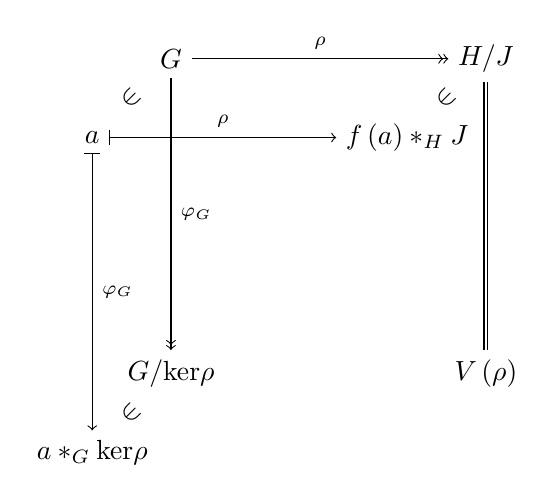
\begin{tikzpicture}[auto]
    \node[rotate=45] (x) at (4.5, 4.5) {$\in $};
    \node[rotate=45] (x) at (0.5, 0.5) {$\in $};
    \node[rotate=45] (x) at (0.5, 4.5) {$\in $};
    \node (c) at (4, 4) {$f\left( a\right) *_H J$};
    \node (e) at (5, 1) {$V\left( \rho \right) $};
    \node (g) at (5, 5) {$H/J$};
    \node (i) at (0, 0) {$a*_G {\rm ker} \rho $};
    \node (j) at (0, 4) {$a$};
    \node (k) at (1, 1) {$G/{\rm ker} \rho $};
    \node (l) at (1, 5) {$G$};
    \draw [->>] (l) to node {$\scriptstyle \rho $} (g);
    \draw [double distance=1pt] (g) to node {} (e);
    \draw [|->] (j) to node {$\scriptstyle \rho $} (c);
    \draw [|->] (j) to node {$\scriptstyle \varphi_G $} (i);
    \draw [->>] (l) to node {$\scriptstyle \varphi_G $} (k);
  \end{tikzpicture} 
\end{center}
$\ker\rho = I$が成り立つことに注意すれば、群準同型定理より次のようになるので、
\begin{center}
  \begin{tikzpicture}[auto]
    \node[rotate=45] (x) at (4.5, 4.5) {$\in $};
    \node[rotate=45] (x) at (0.5, 0.5) {$\in $};
    \node[rotate=45] (x) at (0.5, 4.5) {$\in $};
    \node (c) at (4, 4) {$f\left( a\right) *_H J$};
    \node (e) at (5, 1) {$H/J$};
    \node (g) at (5, 5) {$H/J$};
    \node (i) at (0, 0) {$a*_G I$};
    \node (j) at (0, 4) {$a$};
    \node (k) at (1, 1) {$G/I$};
    \node (l) at (1, 5) {$G$};
    \draw [->>] (l) to node {$\scriptstyle \rho $} (g);
    \draw [double distance=1pt] (g) to node {} (e);
    \draw [|->] (j) to node {$\scriptstyle \rho $} (c);
    \draw [|->] (j) to node {$\scriptstyle \varphi_G $} (i);
    \draw [->>] (l) to node {$\scriptstyle \varphi_G $} (k);
    \draw [>->>] (k) to node {} (e);
  \end{tikzpicture} 
\end{center}
$\left( {G}/{I},*_{G} \right) \cong \left( {H}/{J},*_{H} \right)$が成り立つ。
\end{proof}
\begin{thm}[第2群同型定理]\label{3.1.2.14}
群$(G,*)$の部分群$(H,*)$、正規部分群$(N,*)$が与えられたとする。このとき、次のことが成り立つ。
\begin{itemize}
\item
  群$(H*N,*)$はその群$(G,*)$の部分群である。
\item
  群$(H \cap N,*)$はその部分群$(H,*)$の正規部分群である、即ち、$(H \cap N,*) \trianglelefteq (H,*)$が成り立つ。
\item
  $\left( {H}/{(H \cap N)},* \right) \cong \left( {(H*N)}/{N},* \right)$が成り立つ。
\end{itemize}\par
この定理を第2群同型定理という。
\end{thm}
\begin{proof}
群$(G,*)$の部分群$(H,*)$、正規部分群$(N,*)$が与えられたとする。その群$(H,*)$自身もその群$(H,*)$の正規部分群であることに注意すれば、次のことが成り立つことは定理\ref{3.1.1.27}と定理\ref{3.1.1.28}より明らかである。
\begin{itemize}
\item
  群$(H*N,*)$はその群$(G,*)$の部分群である。
\item
  群$(H \cap N,*)$はその部分群$(H,*)$の正規部分群である。
\end{itemize}\par
このとき、$\ker f = N$が成り立つような群準同型写像$f$によるその群$(G,*)$の群準同型像$\left( G',*' \right)$が存在する。例えば、その群準同型写像$f$が自然な全射群準同型写像の場合などが挙げられる。ここで、その値域$V\left( f|H \right)$を$H'$とおくと、次のようになる。
\begin{center}
  \begin{tikzpicture}[auto]
    \node (y) at (3, 4) {$\subseteq $};
    \node (y) at (7, 4) {$\subseteq $};
    \node (y) at (7, 0) {$\subseteq $};
    \node (a) at (5, 4) {$V\left( f^{-1} |H'\right) $};
    \node (c) at (2, 4) {$H$};
    \node (d) at (2, 0) {$V\left( f|H\right) $};
    \node (e) at (6, 0) {$H'$};
    \node (i) at (8, 4) {$G$};
    \node (j) at (8, 0) {$G'$};
    \draw [->>] (c) to node {} (d);
    \draw [->>] (i) to node {$\scriptstyle f$} (j);
    \draw [double distance=1pt] (d) to node {} (e);
  \end{tikzpicture} 
\end{center}
$\forall a \in G$に対し、$a \in V\left( f^{- 1}|H' \right)$が成り立つなら、$f(a) \in V\left( f|H \right)$が成り立つので、$\exists h \in H$に対し、$f(a) = f(h)$が成り立つ。ここで、定理\ref{3.1.2.8}より$a \equiv h\ \mathrm{mod}\left( \ker f,* \right)$が成り立つ、即ち、$a \equiv h\ \mathrm{mod}(N,*)$が成り立つので、$h^{- 1}*a \in N$が成り立つ、即ち、次のようになる。
\begin{align*}
h*\left( h^{- 1}*a \right) &= \left( h*h^{- 1} \right)*a\\
&= 1_{(G,*)}*a\\
&= a \in h*N \subseteq H*N
\end{align*}
したがって、$V\left( f^{- 1}|H' \right) \subseteq H*N$が成り立つ。逆に、$\forall a \in G$に対し、$a \in H*N$が成り立つなら、$\exists h \in H\exists n \in N$に対し、$a = h*n$と書かれることができ、このとき、$n \in N = \ker f$が成り立つことに注意すれば、次のようになる。
\begin{align*}
f(a) &= f(h*n)\\
&= f(h)*'f(n)\\
&= f(h)*'1_{\left( G',*' \right)}\\
&= f(h)
\end{align*}
したがって、$f(a) \in V\left( f|H \right)$が得られるので、$a \in V\left( f^{- 1}|H' \right)$が成り立つ。したがって、$V\left( f^{- 1}|H' \right) \supseteq H*N$が成り立つ。以上より、$V\left( f^{- 1}|H' \right) = H*N$が得られ次式のようになる。
\begin{center}
  \begin{tikzpicture}[auto]
    \node (y) at (7, 4) {$\subseteq $};
    \node (y) at (7, 0) {$\subseteq $};
    \node (a) at (5, 4) {$V\left( f^{-1} |H'\right) $};
    \node (c) at (2, 4) {$H*N$};
    \node (e) at (6, 0) {$H'$};
    \node (i) at (8, 4) {$G$};
    \node (j) at (8, 0) {$G'$};
    \draw [->>] (i) to node {$\scriptstyle f$} (j);
    \draw [double distance=1pt] (c) to node {} (a);
  \end{tikzpicture} 
\end{center}
ここで、当然ながら$N \subseteq H*N$が成り立つので、第1群同型定理より次式のようになるので、
\begin{center}
  \begin{tikzpicture}[auto]
    \node (y) at (1, 4) {$\subseteq $};
    \node (y) at (7, 4) {$\subseteq $};
    \node (y) at (7, 0) {$\subseteq $};
    \node (a) at (5, 4) {$V\left( f^{-1} |H'\right) $};
    \node (c) at (2, 4) {$H*N$};
    \node (e) at (6, 0) {$H'$};
    \node (f) at (12, 4) {$\left( H*N\right) /N$};
    \node (i) at (8, 4) {$G$};
    \node (j) at (8, 0) {$G'$};
    \node (k) at (0, 4) {$N$};
    \draw [>->>] (f) to node {} (e);
    \draw [->>] (i) to node {$\scriptstyle f$} (j);
    \draw [double distance=1pt] (c) to node {} (a);
    \draw [->>] (c)[bend left=10] to node {} (f);
  \end{tikzpicture} 
\end{center}
$\left( {(H*N)}/{\ker f},* \right) = \left( {(H*N)}/{N},* \right) \cong \left( H',*' \right)$が成り立つ。\par
また、写像$f':H \rightarrow V\left( f|H \right);h \mapsto f(h)$は全射群準同型写像で、$\forall h \in G$に対し、$h \in \ker f'$が成り立つならそのときに限り、$h \in H$が成り立つかつ、$h \in \ker f$が成り立ち、したがって、これが成り立つならそのときに限り、$h \in H \cap N$が成り立つので、$\ker f' = H \cap N$が成り立つ。ここで、$(H,*) \trianglelefteq (H,*)$に注意すれば、定理\ref{3.1.1.28}より$(H \cap N,*) \trianglelefteq (H,*)$で第1群同型定理より次式のようになるので、
\begin{center}
  \begin{tikzpicture}[auto]
    \node (y) at (1, 4) {$\subseteq $};
    \node (c) at (2, 4) {$H$};
    \node (e) at (6, 0) {$H'$};
    \node (f) at (12, 4) {$H/\left( H\cap N\right) $};
    \node (i) at (8, 4) {$H$};
    \node (j) at (8, 0) {$V\left( f|H\right) $};
    \node (k) at (0, 4) {$H\cap N$};
    \draw [>->>] (f) to node {} (e);
    \draw [->>] (i) to node {$\scriptstyle f'$} (j);
    \draw [double distance=1pt] (c) to node {} (i);
    \draw [double distance=1pt] (e) to node {} (j);
    \draw [->>] (c)[bend left=10] to node {} (f);
  \end{tikzpicture} 
\end{center}
$\left( {H}/{(H \cap N)},* \right) \cong \left( H',*' \right)$が成り立つ。\par
以上より、$\left( {H}/{(H \cap N)},* \right) \cong \left( H',*' \right) \cong \left( {(H*N)}/{N},* \right)$が得られたので、$\left( {H}/{(H \cap N)},* \right) \cong \left( {(H*N)}/{N},* \right)$が成り立つ。
\end{proof}
\begin{thm}\label{3.1.2.15}
群々$\left( G,*_{G} \right)$、$\left( H,*_{H} \right)$の間の群準同型写像$f:G \rightarrow H$、その群$\left( G,*_{G} \right)$の正規部分群$\left( N,*_{G} \right)$が与えられたとき、$N \subseteq \ker f$が成り立つならそのときに限り、次式のような群準同型写像$\overline{f}$が存在する。
\begin{align*}
\overline{f}:{G}/{N} \rightarrow H;a*_{G}N \mapsto f(a)
\end{align*}
\end{thm}
\begin{proof}
群々$\left( G,*_{G} \right)$、$\left( H,*_{H} \right)$の間の群準同型写像$f:G \rightarrow H$、その群$\left( G,*_{G} \right)$の正規部分群$\left( N,*_{G} \right)$が与えられたとき、$N \subseteq \ker f$が成り立つなら、$\forall a,b \in N$に対し、$a*_{G}b^{- 1} \in N \subseteq \ker f$が成り立つので、次のようになる。
\begin{align*}
f(a) &= f(a)*_{H}1_{\left( H,*_{H} \right)}\\
&= f(a)*_{H}{f(b)}^{- 1}*_{H}f(b)\\
&= f(a)*_{H}f\left( b^{- 1} \right)*_{H}f(b)\\
&= f\left( a*_{G}b^{- 1} \right)*_{H}f(b)\\
&= 1_{\left( H,*_{H} \right)}*_{H}f(b)\\
&= f(b)
\end{align*}
したがって、$\forall f(a),f(b) \in H$に対し、$f(a) \neq f(b)$が成り立つなら、$a*_{G}b^{- 1} \notin N$が成り立つので、定理\ref{3.1.1.18}より$a*_{G}N \neq b*_{G}N$が成り立つ。対偶律により$\forall a*_{G}N,b*_{G}N \in {G}/{N}$に対し、$a*_{G}N = b*_{G}N$が成り立つなら、$f(a) = f(b)$が成り立つので、次式のような写像$\overline{f}$が存在する。
\begin{align*}
\overline{f}:{G}/{N} \rightarrow H;a*_{G}N \mapsto f(a)
\end{align*}
ここで、$\forall a*_{G}N,b*_{G}N \in {G}/{N}$に対し、定理\ref{3.1.1.29}より次のようになるので、
\begin{align*}
\overline{f}\left( a*_{G}N*_{G}b*_{G}N \right) &= \overline{f}\left( a*_{G}b*_{G}N \right)\\
&= f\left( a*_{G}b \right)\\
&= f(a)*_{H}f(b)\\
&= \overline{f}\left( a*_{G}N \right)*_{H}\overline{f}\left( b*_{G}N \right)
\end{align*}
その写像$\overline{f}$は群準同型写像である。\par
逆に、次式のような群準同型写像$\overline{f}$が存在するなら、
\begin{align*}
\overline{f}:{G}/{N} \rightarrow H;a*_{G}N \mapsto f(a)
\end{align*}
自然な全射群準同型写像$\varphi_{G}:G \twoheadrightarrow {G}/{N};a \mapsto a*_{G}N$を用いれば、定義より明らかに$f = \overline{f} \circ \varphi_{G}$が成り立つので、$\forall n \in N$に対し、定理\ref{3.1.2.1}より次のようになる。
\begin{align*}
f(h) &= \overline{f} \circ \varphi_{G}(n)\\
&= \overline{f}\left( n*_{G}N \right)\\
&= \overline{f}(N)\\
&= \overline{f}\left( 1_{\left( G,*_{G} \right)}*_{G}N \right)\\
&= f\left( 1_{\left( G,*_{G} \right)} \right)\\
&= 1_{\left( H,*_{H} \right)}
\end{align*}
これにより、$n \in \ker f$が成り立つので、$N \subseteq \ker f$が成り立つ。
\end{proof}
\begin{thm}[第3群同型定理]\label{3.1.2.16}
群$(G,*)$の正規部分群たち$(M,*)$、$(N,*)$が与えられ、$M \subseteq N$が成り立つとき、$\left( {G}/{N},* \right) \cong \left( {\left( {G}/{M} \right)}/{(N/M)},* \right)$が成り立つ。\par
この定理を第3群同型定理という。
\end{thm}
\begin{proof}
群$(G,*)$の正規部分群たち$(M,*)$、$(N,*)$が与えられ、$M \subseteq N$が成り立つとき、自然な全射群準同型写像$\varphi:G \twoheadrightarrow {G}/{N};a \mapsto a*N$を用いれば、定理\ref{3.1.2.7}より$M \subseteq N = \ker\varphi$が成り立つので、定理\ref{3.1.2.15}より次式のような群準同型写像$\overline{f}$が存在して
\begin{align*}
\overline{\varphi}:{G}/{M} \rightarrow {G}/{N};a*M \mapsto \varphi(a) = a*N
\end{align*}
次式のようになる。
\begin{center}
  \begin{tikzpicture}[auto]
    \node (a) at (0, 4) {$G/M$};
    \node (b) at (4, 4) {$G/N$};
    \node (c) at (0, 0) {$\left( G/M\right) /{\rm ker} \bar{\varphi } $};
    \node (d) at (4, 0) {$V\left( \bar{\varphi } |G/M\right) $};
    \node (e) at (4, 2) {\rotatebox{90}{$\subseteq $} };
    \node (f) at (2, 2) {$G$};
    \draw [->>] (f) to node {$\scriptstyle \varphi $} (b);
    \draw [->] (a) to node {$\scriptstyle \bar{\varphi } $} (b);
    \draw [->>] (a) to node {} (c);
  \end{tikzpicture} 
\end{center}
ここで、$\forall a*M \in \ker\overline{\varphi}$に対し、$\overline{\varphi}(a*M) = a*N = N$が成り立つならそのときに限り、$a \in N$が成り立つので、$a*M \in {N}/{M}$が成り立つ。したがって、$\ker\overline{\varphi} = {N}/{M}$が得られる。そこで、群準同型定理より次式のような写像$g:{\left( {G}/{M} \right)}/{\left( {N}/{M} \right)}\overset{\sim}{\rightarrow}V\left( \overline{\varphi}|{G}/{N} \right)$が存在する。
\begin{center}
  \begin{tikzpicture}[auto]
    \node (a) at (0, 4) {$G/M$};
    \node (b) at (4, 4) {$G/N$};
    \node (c) at (0, 0) {$\left( G/M\right) /\left( N/M\right) $};
    \node (d) at (4, 0) {$V\left( \bar{\varphi } |G/M\right) $};
    \node (e) at (4, 2) {\rotatebox{90}{$\subseteq $} };
    \node (f) at (2, 2) {$G$};
    \draw [->>] (f) to node {$\scriptstyle \varphi $} (b);
    \draw [->] (a) to node {$\scriptstyle \bar{\varphi } $} (b);
    \draw [->>] (a) to node {} (c);
    \draw [>->>] (c) to node {$\scriptstyle g$} (d);
  \end{tikzpicture} 
\end{center}
一方で、次式のような自然な全射群準同型写像$\varphi':G \twoheadrightarrow {G}/{M};a \mapsto a*M$が考えられれば、次のようになり
\begin{center}
  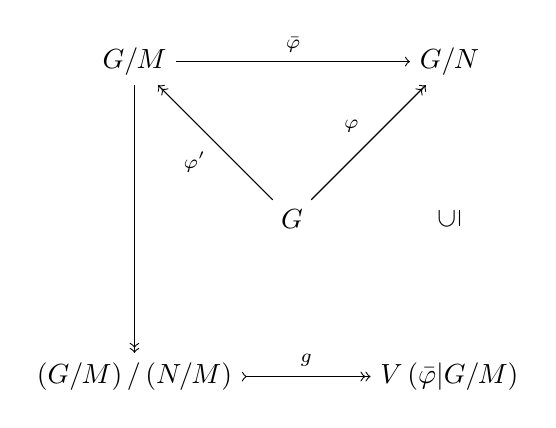
\begin{tikzpicture}[auto]
    \node (a) at (0, 4) {$G/M$};
    \node (b) at (4, 4) {$G/N$};
    \node (c) at (0, 0) {$\left( G/M\right) /\left( N/M\right) $};
    \node (d) at (4, 0) {$V\left( \bar{\varphi } |G/M\right) $};
    \node (e) at (4, 2) {\rotatebox{90}{$\subseteq $} };
    \node (f) at (2, 2) {$G$};
    \draw [->>] (f) to node {$\scriptstyle \varphi' $} (a);
    \draw [->>] (f) to node {$\scriptstyle \varphi $} (b);
    \draw [->] (a) to node {$\scriptstyle \bar{\varphi } $} (b);
    \draw [->>] (a) to node {} (c);
    \draw [>->>] (c) to node {$\scriptstyle g$} (d);
  \end{tikzpicture} 
\end{center}
$\varphi = \overline{\varphi} \circ \varphi'$が成り立つので、$\forall\overline{\varphi}(a*M) \in V\left( \overline{\varphi}|{G}/{M} \right)$に対し、次のようになるので、
\begin{align*}
\overline{\varphi}(a*M) &= \overline{\varphi}\left( \varphi'(a) \right)\\
&= \overline{\varphi} \circ \varphi'(a)\\
&= \varphi(a) \in V(\varphi)
\end{align*}
その写像$\varphi$が全射であることに注意すれば、$\overline{\varphi}(a*M) \in V\left( \overline{\varphi}|{G}/{M} \right)$が成り立つならそのときに限り、$\varphi(a) \in {G}/{N}$が成り立つので、次式のようになる。
\begin{center}
  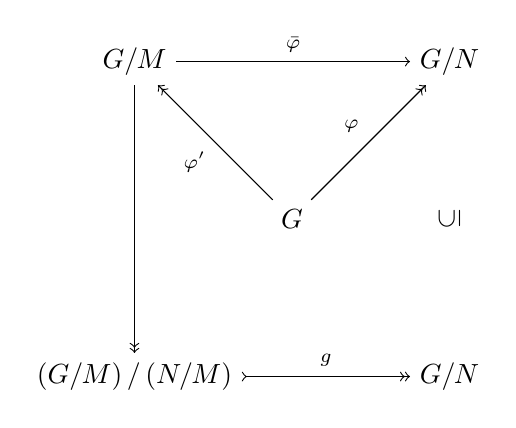
\begin{tikzpicture}[auto]
    \node (a) at (0, 4) {$G/M$};
    \node (b) at (4, 4) {$G/N$};
    \node (c) at (0, 0) {$\left( G/M\right) /\left( N/M\right) $};
    \node (d) at (4, 0) {$G/N$};
    \node (e) at (4, 2) {\rotatebox{90}{$\subseteq $} };
    \node (f) at (2, 2) {$G$};
    \draw [->>] (f) to node {$\scriptstyle \varphi' $} (a);
    \draw [->>] (f) to node {$\scriptstyle \varphi $} (b);
    \draw [->] (a) to node {$\scriptstyle \bar{\varphi } $} (b);
    \draw [->>] (a) to node {} (c);
    \draw [>->>] (c) to node {$\scriptstyle g$} (d);
  \end{tikzpicture} 
\end{center}
したがって、$\left( {G}/{N},* \right) \cong \left( {\left( {G}/{M} \right)}/{(N/M)},* \right)$が成り立つ。
\end{proof}
\begin{thebibliography}{50}
  \bibitem{1}
  松坂和夫, 代数系入門, 岩波書店, 1976. 新装版第2刷 p65-71 ISBN978-4-00-029873-5
  \bibitem{2}
  よしいず. "群の同型定理". MATHEMATICS.PDF. \url{https://mathematics-pdf.com/pdf/grp_iso_thm.pdf} (2021-8-8 15:30 取得)
  \bibitem{3}
  花木章秀. "群論". 信州大学. \url{http://math.shinshu-u.ac.jp/~hanaki/edu/group/group2011pre.pdf} (2021-8-8 16:00 取得)
\end{thebibliography}
\end{document}
